\documentclass[10pt, a4paper]{article}
\usepackage[utf8]{inputenc}
% especifico márgenes manualmente
\usepackage[paper=a4paper, margin=2cm]{geometry}
% codificación ISO-8859-1
%\usepackage[latin1]{inputenc}
% separación silábica en castellano
\usepackage[spanish]{babel}
\usepackage{algorithm}
\usepackage{algpseudocode}
\usepackage{caratula/caratula}
\graphicspath{ {images/} }
%\usepackage{tikz}
%\usepackage{tikz-qtree}
%\usepackage{framed}
%\usepackage{array}
%\usepackage{tabular}

\begin{document}

\titulo{Trabajo Práctico \#1}
\fecha{Abril de 2018}
\materia{Algoritmos y Estructuras de Datos III}

\integrante{Eric Brandwein}{349/16}{brandweineric@gmail.com}
% \integrante{Pepe Sánchez}{444/12}{pepe@gmail.com}
% \integrante{Roberto Carlos}{111/10}{roberto@gmail.com}


\maketitle

% compilar 2 veces para actualizar las referencias
\tableofcontents

\pagebreak
%\newpage


\section{Descripci\'on del problema}

%\begin{framed}
El problema a resolver en este informe será el ya conocido problema de la mochila, o "Knapsack problem", en inglés. Su enunciado dice así: \\
Dado un conjunto de $n$ ítems $S$, cada uno con un tamaño asociado $w_i$ y un beneficio asociado $p_i$, y una mochiula con una capacidad asociada $W$, encontrar el subconjunto de ítems de $S$ que maximice el beneficio total sin exceder la capacidad de la mochila. Es decir, encontrar $R \subseteq S$ tal que $\sum_{i \in R} p_i$ sea máxima y se cumpla $\sum_{i \in R} w_i \leq W$. Asumiremos que todos los valores mencionados son enteros no negativos.\par

Para entender mejor el problema, mostraremos un ejemplo: \par
Imaginemos que poseemos una mochila con capacidad 25, y que poseemos 5 ítems, cada uno con su tamaño y beneficio asociados de esta forma: \\
\begin{tabular}{c|c|c}
	ítem & tamaño & beneficio \\ \hline
	1 & 10 & 5 \\
	2 & 15 & 4 \\
	3 & 5 & 13 \\
	4 & 10 & 8 \\
	5 & 5 & 8
\end{tabular} \\
La combinación de ítems que maximizará el beneficio sin pasarse de la capacidad de la mochila será el conjunto $\{3, 4, 5\}$, que juntos suman un tamaño de $5 + 10 + 5 = 20$ y un beneficio de $13 + 8 + 8 = 29$. Cualquier otra combinación de los ítems que poseemos o no entrará en la mochila por tener un tamaño total mayor a la capacidad, o tendrá un beneficio total menor o igual al beneficio alcanzado con la solución dada. \par

Algorítmicamente, desarrollaremos cuatro maneras de llegar a la solución para cualquier conjunto de argumentos. Demostraremos la correctitud de cada una, y luego las compararemos tanto en términos de complejidad teórica como con comprobaciones empíricas. Las estrategias de programación que utilizaremos son:
\begin{itemize}
	\item Fuerza Bruta
	\item Meet in the Middle
	\item Backtracking
	\item Programación Dinámica
\end{itemize}

\section{Fuerza Bruta}
\subsection{Descripción}
Este algoritmo resuelve el problema comparando todas las combinaciones de ítems entre sí.
Las mismas se generan una tras otra. Cada vez que se genera una combinación de ítems, se calcula su beneficio y su tamaño total. Si el tamaño es mayor a la capacidad de la mochila, la combinación se descarta. Si no, se compara el beneficio total de la solución actual con el mayor beneficio alcanzado hasta el momento, y se mantiene el mayor beneficio entre los dos, para ser comparado más tarde con la próxima posible solución. Si para el momento de la comparación no se había encontrado todavía una combinación que entrase en la mochila, el mayor beneficio encontrado hasta el momento será igual a cero. Podemos comenzar asumiendo un beneficio cero porque sabemos que siempre existe por lo menos una combinación de ítems con este beneficio; particularmente, la combinación en la que no se pone ningún item en la mochila posee este beneficio total.\par
En el momento en el que ya se hubieron recorrido todas las combinaciones, el resultado será el mayor beneficio encontrado. \par

\subsection{Pseudocódigo}

A continuación se muestra el pseudocódigo para el algoritmo mencionado, que utiliza las funciones \\
\texttt{primerCombinacion} y \texttt{proximaCombinacion} para iterar sobre las combinaciones posibles de ítems, y \\
\texttt{beneficioDeCombinacion}, que suma los beneficios de todos los ítems presentes en la combinación actual.

\pagebreak
\begin{algorithm}
\caption{Fuerza Bruta}
\begin{algorithmic}[1]
\Function{fuerzaBruta}{$capacidad, items$}
	\State $mayorBeneficio \gets 0$
	\State $combinacionActual \gets $\Call{primerCombinacion}{items}
	\While{\Call{combinacionValida?}{combinacionActual}}
		\State $tamanioActual \gets $\Call{tamanioDeCombinacion}{combinacionActual}
		\If{$tamanioActual \leq capacidad$}
			\State $beneficioActual \gets $\Call{beneficioDeCombinacion}{combinacionActual}
			\State $mayorBeneficio \gets max(beneficioActual, mayorBeneficio)$
		\EndIf

		\State $combinacionActual \gets $\Call{proximaCombinacion}{combinacionActual}
	\EndWhile
	\State \Return $mayorBeneficio$
\EndFunction
\end{algorithmic}
\end{algorithm}

\subsection{Correctitud}
Sabemos que no hay un mejor resultado que el devuelto porque si existiese una combinación con beneficio mayor, la hubiésemos encontrado y guardado. Y sabemos que hay una combinación con ese beneficio porque solo guardamos el resultado si encontramos una combinación con ese beneficio. Por ende, el resultado devuelto es el correcto. \par

\subsection{Complejidad}
Para calcular la complejidad, seguiremos el pseudocódigo anterior paso a paso. Tomaremos $n$ como la cantidad de ítems que se pasan como parámetro.\par
\begin{itemize}
	\item Las líneas 2 y 12 tienen una complejidad de $O(1)$.
	\item La línea 3 llama a la función $primerCombinacion$, que devuelve una combinación de ítems en $O(n)$.
	\item En la línea 4 comienza el bucle que recorrerá todas las combinaciones de ítems. La cantidad de combinaciones de ítems será $2^n$, ya que cada por cada ítem hay dos posibilidades: que esté adentro de la mochila o que no esté. Además, en la misma linea se llama a la función $combinacionValida?$, la cual tiene una complejidad de $O(n)$. Así que, en un principio, este bucle tiene una complejidad de $O(2^n * n)$.
	\item La línea 5 llama a $tamanioDeCombinacion$, que calcula la suma de todos los tamaños de cada ítem presente en la combinación actual. Tiene una complejidad de $O(n)$, la cual no suma a la complejidad ya establecida del bucle de $O(2^n * n)$.
	\item La línea 6 realiza una comparación simple, de complejidad $O(1)$. Lo mismo sucede con la línea 8, que solo calcula un máximo.
	\item La línea 7 hace algo parecido a la línea 5, pero en vez de sumar los tamaños, suma los beneficios. Otra vez, no aumenta la complejidad ya establecida para el bucle.
	\item La línea 10 calcula la próxima combinación de ítems. Esto se puede lograr con una complejidad de $O(n)$, si tomamos una combinación de items como un número binario de longitud $n$, con los $1$ significando que el ítem está presente. La primera combinación podría ser la vacía, y cada vez que se avanza a la siguiente combinación, lo único que se hace es sumarle uno al número binario que representaba a la combinación anterior. Esta línea tampoco aumenta la complejidad del bucle.
\end{itemize}
Gracias a éste análisis, podemos ahora sumar las complejidades de cada línea, y encontrar la complejidad final del algoritmo: $2 * O(1) + O(n) + O(2^n * 3n) = O(2^n * n)$.


\section{Meet in the Middle}
\subsection{Descripción}
Este algoritmo toma ventaja de la búsqueda binaria para mejorar la complejidad del algoritmo de fuerza bruta. A grandes rasgos, el algoritmo sigue estos pasos: \\
\begin{enumerate}
	\item Divide al conjunto de ítems en dos mitades;
	\item Encuentra los tamaños y beneficios del conjunto de partes de cada una, sacando las partes que tengan un tamaño mayor a la capacidad de la mochila;
	\item Ordena las partes de la segunda mitad de menor a mayor en tamaño, y si hay dos partes con el mismo tamaño, las ordena de mayor a menor en beneficio;
	\item Saca las partes de la segunda mitad para las que exista otra parte con menor o igual tamaño e igual o mayor beneficio;
	\item Por cada parte del primer conjunto, se encuentra, con una búsqueda binaria por tamaño en el segundo conjunto, la parte que mejor llene la restante capacidad de la mochila. Es decir, la parte del segundo conjunto que tenga el mayor tamaño de las partes que, sumando el tamaño de la parte del primer conjunto, no sobrepasen la capacidad de la mochila;
	\item Se suman los beneficios de la parte encontrada con la parte actual del primer conjunto;
	\item Se encuentra el mayor beneficio entre las partes restantes, y se llega al resultado deseado.
\end{enumerate}


\subsection{Pseudocódigo}
\begin{algorithm}
\caption{Meet in the Middle}
\begin{algorithmic}[1]
\Function{meetInTheMiddle}{$capacidad, items$}
	\State $primerMitad \gets items[0..items.size / 2]$
	\State $segundaMitad \gets items[items.size / 2..items.size]$

	\State $primerasPartes \gets $ \Call{conjuntoDePartes}{$primerMitad, capacidad$}
	\State $segundasPartes \gets $ \Call{conjuntoDePartes}{$segundaMitad, capacidad$}

	\State $segundasPartes \gets $ \Call{ordenarPartes}{$segundasPartes$}
	\State $segundasPartes \gets $ \Call{sacarInservibles}{$segundasPartes$}

	\State $posiblesSoluciones \gets $ \Call{combinar}{$primerasPartes, segundasPartes, capacidad$}

	\State $mayorBeneficio \gets $ \Call{encontrarMayorBeneficio}{$posiblesSoluciones$}
	\State \Return $mayorBeneficio$
\EndFunction
\\
\Function{conjuntoDePartes}{$items, capacidad$}
	\State $partes \gets \{parte(beneficio=0, tamano=0)\}$
	\ForAll{$itemActual \in items$}
		\State $partesAnteriores \gets partes$
		\ForAll{$parteActual \in partesAnteriores$}
			\State $nuevaParte \gets parteActual + itemActual$
			\If{$nuevaParte.tamano <= capacidad$}
				\State $partes.pushBack(nuevaParte)$
			\EndIf
		\EndFor
	\EndFor
	\State \Return $partes$
\EndFunction
\\
\Function{sacarInservibles}{$partesOriginales$}

	\State $partes \gets \{parte(beneficio=0, tamano=0)\}$
	\ForAll{$parteActual \in partesOriginales$}
		\State $parteAnterior \gets partes.back()$
		\If{$parteAnterior.beneficio < parteActual.beneficio$}
			\State $partes.pushBack(parteActual)$
		\EndIf
	\EndFor

	\State \Return $partes$
\EndFunction
\algstore{meet}
\end{algorithmic}
\end{algorithm}

\begin{algorithm}
\begin{algorithmic}[1]

\algrestore{meet}
\Function{combinar}{$primerasPartes, segundasPartes, capacidad$}
	\State $partesCombinadas \gets \{\}$
	\ForAll{$parteActual \in primerasPartes$}
		\State $parteResultante \gets parteActual$
		\State $tamanoRestante \gets capacidad - parteActual.tamano$
		\State $segundaParteComplementaria \gets$\Call{buscarParteConTamano}{$segundasPartes, tamanoRestante$}
		\If{$segundaParteComplementaria != null$}
			\State $parteResultante \gets parteResultante + segundaParteComplementaria$
		\EndIf
		\State $partesCombinadas.pushBack(parteResultante)$
	\EndFor
	\State \Return $partesCombinadas$
\EndFunction
\end{algorithmic}
\end{algorithm}
\pagebreak
\subsection{Correctitud}
%Sabemos que por lo menos uno de los conjuntos de ítems es la solución, porque sabemos que siempre por lo menos el conjunto vacío entra en la mochila.
%Demostraremos la correctitud siguiendo los pasos de la descripción.
Veamos que el valor devuelto es en realidad la solución del problema. \par
Al principio, encontramos el conjunto de partes de cada una de las dos mitades, con un bucle que recorre todos los items. Por cada item, se suma su tamaño y su beneficio a todas las partes que ya se habían creado, y se generan partes nuevas. Así, tenemos todas las partes que se pueden armar con todos los items anteriores, más todas las mismas pero con el nuevo ítem. Cuando terminamos de recorrer todos los ítems, obtenemos todas las partes posibles de esa mitad, excepto las que sobrepasan la capacidad de la mochila, las cuales removemos.\par
Luego, ordenamos las partes de menor a mayor en tamaño, y si dos combinaciones tienen el mismo tamaño, ordenamos de mayor a menor en beneficio. Hacer esto nos simplifica la tarea de remover las partes que llamamos ``inservibles". Son las partes para las cuales existe una parte en la misma mitad que sea mejor, es decir, que tenga menor o igual tamaño y mayor o igual beneficio. Si existe tal parte, la misma aprovecha mejor o igual el mismo tamaño, y por lo tanto no es necesario conservar las que lo utilizan peor. En el caso especial en la que hay dos combinaciones con el mismo beneficio y el mismo tamaño, se puede conservar cualquiera de las dos, por ejemplo, la que aparezca primero cuando recorremos el conjunto.\par
Para ver cómo nos simplifica la filtración del arreglo de partes el haberlas ordenado de esta forma, imaginemos que, por cada combinación, partimos el arreglo en dos: el arreglo de las combinaciones posteriores, y el de las anteriores. Asumamos que ya habíamos filtrado el arreglo anterior a esta combinación. Este arreglo total estaba ordenado por tamaño, así que el último elemento será el de mayor tamaño, pero tendrá menor o igual tamaño que la combinación actual. También será el de mayor beneficio, porque si hubiese uno de mayor beneficio con menor tamaño, este sería inservible. Ahora, por cómo habíamos ordenado el arreglo, las combinaciones posteriores a la actual o tienen mayor tamaño, o tienen igual tamaño pero menor o igual beneficio. Esto quiere decir que ninguna hará que esta sea inservible. Llegamos a la conclusión de que solamente las combinaciones anteriores pueden ser mejores. Y, como la última combinación de la mitad anterior tiene mayor beneficio que todas las otras, y menor o igual tamaño que la combinación actual, solo hace falta comparar con ella el beneficio de la combinación actual para llegar a la decisión de si es inservible o no. Como esto ocurre con cada una de las combinaciones, no nos hace falta hacer más de una comparación por combinación del conjunto.\par
Sacar los inservibles hace que no pueda haber dos combinaciones con el mismo tamaño en la segunda mitad. Esto se debe a que, si hubiese dos con el mismo tamaño, alguna tendría menor o igual beneficio que la otra, y por lo tanto la habríamos sacado. Además, esa mitad está ordenada por beneficio, ya que si hubiese uno posterior a otro con mayor beneficio, el anterior tendría menor tamaño, lo que haría que este sea inservible.\par
Ahora queremos combinar las combinaciones de los conjuntos para llegar a posibles soluciones. Por cada combinación en el primer conjunto, encontramos, con una búsqueda binaria, la que tenga mayor tamaño en la segunda mitad sin pasarse de la capacidad total si sumamos los tamaños. Sabemos que la misma será la que mayor beneficio nos pueda aportar para la combinación actual, por el hecho de que el arreglo está ordenado por tamaño y por beneficio. Así, obtenemos la mejor combinación total de ítems para cada semi-combinación de ítems de la primer mitad\par
Tenemos ahora las mejores combinaciones de ítems totales, y para resolver el problema encontramos la que tenga mayor beneficio de todas, y devolvemos su valor.

\subsection{Complejidad}
Para llegar a una cota de la complejidad de este algoritmo, analizaremos cada función que utililza, y luego las uniremos.\par
Comenzando, en el pseudocódigo mostrado, por la función $conjuntoDePartes$, podemos ver que realiza la porción de código interior a los dos bucles una cantidad de veces igual a la cantidad de combinaciones posibles con esos ítems. En la misma, se llaman a todas operaciones con complejidad $O(1)$, excepto la llamada a $pushBack$, que, si utilizamos un $vector$ de C++, tiene una complejidad de $O(1)$ amortizada. Por estas razones, la función tiene una complejidad perteneciente a $O(2^n)$, siendo $n$ la cantidad de ítems. Llamamos dos veces a esta función con una cantidad de ítems igual a la mitad de la cantidad original, lo que nos da una complejidad inicial de $O(2^{n/2})$, siendo $n$ la cantidad de ítems originales.\par
Siguiendo con el pseudocódigo, la función $sacarInservibles$ recorre todas las combinaciones o partes del conjunto de partes pasado como parámetro. Por cada una, otra vez, llama a todas operaciones con complejidad $O(1)$ u $O(1)$ amortizado, con lo que nos queda que la función tiene una complejidad de $O(n)$, siendo $n$ la cantidad de partes. Como la llamamos una sola vez con el conjunto de partes de una sola mitad de los ítems, nos suma $O(2^{n/2})$ a la complejidad inicial.\par
Llegando ya a la función combinar, vemos que recorre cada una de las $primerasPartes$, y realiza adentro una búsqueda binaria y otras operaciones con complejidad $O(1)$, amortizado o no. Realiza la búsqueda sobre las combinaciones de la segunda mitad. Como cada una de las mitades contiene como máximo $2^{n/2}$ combinaciones, la complejidad resultante es $O(2^{n/2} * \log{}2^{n/2}) = O(2^{n/2} * n/2)$.\par
Ahora sí calcularemos la complejidad del algoritmo en su totalidad. Primero, se parte el conjunto de ítems a la mitad, cosa que se puede hacer en $O(n)$ u $O(1)$, dependiendo de cómo se implemente. Luego, se llama dos veces a $conjuntoDePartes$, y cada una suma $O(2^{n/2})$ a la complejidad. $ordenarPartes$, si se utiliza, por ejemplo, merge-sort, puede tener una complejidad de $O(2^{n/2} * \log{}2^{n/2}) = O(2^{n/2} * n/2)$. Seguimos con $sacarInservibles$, la cual vimos que tiene una complejidad de $O(2^{n/2})$, y $combinar$, que vimos que nos suma $O(2^{n/2} * n/2)$. Por último, $encontrarMayorBeneficio$ simplemente recorre todas las posibles soluciones, que, como hay una posible solución por combinación en el primer conjunto de partes, nos suma solamente $O(2^{n/2})$.\par
Sumando todas estas complejidades diferentes llegamos a $O(n) + 2 * O(2^{n/2}) + O(2^{n/2} * n/2) + O(2^{n/2}) + O(2^{n/2} * n/2) + O(2^{n/2}) = O(2^{n/2} * n)$.

\section{Backtracking}
\subsection{Descripción}
En el algoritmo de Backtracking armaremos un árbol de decisiones, cada una especificando si incluimos un ítem en particular en la combinación actual o no. Haremos la decisión para el primer ítem, luego para el segundo ítem, y así. Cuando lleguemos a una hoja del árbol, compararemos el beneficio de los ítems que decidimos incluir en la combinación con el mejor beneficio encontrado hasta el momento, y nos quedaremos con el mejor.\par
A diferencia del algoritmo de Fuerza Bruta, para no probar con combinaciones de ítems que ya sabemos de antemano que no serán óptimas o que directamente no entrarán en la mochila, haremos podas de factibilidad y de optimalidad, es decir, cuando se cumplan algunas condiciones particulares, no seguiremos decidiendo en la rama en la que estamos, sino que pasaremos a una rama diferente.\par
La poda por factibilidad es simple: mientras vamos haciendo decisiones sobre los ítems, vamos sumando los tamaños de los que agregamos. Cuando el tamaño sumado sobrepasa la capacidad de la mochila, sabemos que esta rama no es factible, así que pasamos a la siguiente. El pseudocódigo de la función que determina si una rama es factible sería algo como lo siguiente:

\begin{algorithm}
\begin{algorithmic}[1]

\Function{podaPorFactibilidad}{$capacidad, tamanoActual, nuevoItem$}
	\State \Return $tamanoActual + nuevoItem.tamano \leq capacidad$
\EndFunction

\end{algorithmic}
\end{algorithm}

La poda por optimalidad, en cambio, es un poco más elaborada. Antes de comenzar a recorrer el árbol, ordenamos los ítems de mayor a menor según el valor que toma su $beneficio/tamano$; su ``ratio". Mientras recorremos el árbol, vamos sumando los beneficios de los ítems que agregamos a la combinación. Además, cada vez que debamos tomar a una decisión, nos fijamos si llenar la capacidad restante de la mochila con un ítem hipotético que tenga el mismo ratio que el ítem actual mejora el beneficio de la mejor solución encontrada hasta el momento. Si no lo mejora, ya sabemos que cualquier combinación de ítems siguientes no superará en beneficio a la solución que habíamos encontrado antes, y por lo tanto esta rama ya no nos sirve, lo que nos hace pasar a la siguiente. Esto se calcula con el siguiente pseudocódigo:\par

\begin{algorithm}
\begin{algorithmic}[1]

\Function{podaPorOptimalidad}{$capacidad, tamanoActual, beneficioActual, nuevoItem, mejorBeneficio$}
	\State $beneficioHipotetico \gets beneficioActual$
	\State $capacidadRestante \gets capacidad - tamanoActual$
	\State $beneficioHipotetico += ( ratio(nuevoItem) * capacidadRestante )$
	\State \Return $beneficioHipotetico > mejorBeneficio$
\EndFunction

\end{algorithmic}
\end{algorithm}

En la función descripta asumimos que la función \texttt{ratio} devuelve un valor infinito si el tamaño del ítem es igual a cero, y que infinito siempre es mayor a cualquier otro valor.\par

Al finalizar, devolvemos el mayor beneficio que hayamos encontrado para una solución factible.\par
Pasaremos a mostrar una corrida hipotética del algoritmo con los valores presentados en el ejemplo de la descripción del problema. La capacidad de la mochila era 25, y la lista de ítems provistos es $[(10, 5), (15, 4), (5, 13),$ $(10, 8), (5, 8)]$, siendo un ítem una tupla $(tamano, beneficio)$.\par
Primero, se ordena la lista por ratio, lo que nos resulta en $[(5, 13), (5, 8), (10, 8), (10, 5), (15, 4)]$. Luego, recorremos el árbol de decisiones, empezando con la decisión de que el primer ítem se encuentra en la combinación que probaremos. Agregando ese item, tomamos su tamaño y su beneficio, y los establecemos como los valores actuales de la combinación actual. Tenemos entonces 5 de tamaño y 13 de beneficio por ahora.\par
Avanzamos a la decisión siguiente, que es la de agregar o no el segundo ítem. Si lo agregásemos, el tamaño de la combinación pasaría a ser 10, y el beneficio 21. Como 10 no se pasa de la capacidad de la mochila, la combinación por ahora pasa la poda de factibilidad. Y la poda por optimalidad por ahora no hace falta chequearla porque no encontramos todavía una posible solución, así que podemos agregar el ítem a la combinación actual.\par
Seguimos con la próxima decisión, que es de agregar el ítem $(10, 8)$. Lo agregamos, por lo mismo que antes, y nos queda un tamaño actual de 20 y un beneficio de 29.\par
Agregar el cuarto ítem haría que no pasásemos la poda por factibildad, así que decidimos no agregarlo. Lo mismo con el quinto ítem, con lo que llegamos a una posible solución que entra en la mochila y tiene beneficio 29. Nos guardamos este valor para después usarlo en la poda por optimalidad.\par
Ahora que llegamos a una hoja del árbol de decisiones, volvemos para atrás hasta encontrar el último ítem que hayamos agregado a la combinación, y probar la combinación de ítems sin ese ítem. Este ítem es el tercero, el $(10, 8)$, y sacándolo nos queda un beneficio de 21 y un tamaño de 10.\par
Ahora tratamos de agregar el cuarto ítem, el $(10, 5)$. Si lo agregásemos, nos quedaría un tamaño de 20, o sea que pasa la poda de factibilidad. Para la poda de optimalidad, calculamos su ratio, que es $5 / 10 = 0.5$, y llenamos el tamaño restante de la mochila con ese ratio. Esto quiere decir que hacemos la cuenta $0.5 * (25 - 10) = 7.5$. Luego, sumamos el valor resultante con el beneficio actual, que sería $21 + 7.5 = 28$. Como 28 es menor al beneficio de la mejor posible solución que encontramos, sabemos que, aunque llenemos la mochila con todos los ítems que quedan, la posible solución no nos va a servir. Por eso, descartamos toda la rama actual, y volvemos a buscar el último ítem que agregamos, que ahora pasa a ser el segundo, el $(5, 8)$.\par
Si siguiésemos con el algoritmo, veríamos que ninguna combinación de ítems factible supera el beneficio que ya encontramos, así que la solución al problema resulta ser 29.\par

%\Tree
%[.{item 1}
%	[.{item 2} [.{item 3} [.{item 4} {item 5} {item 5} ]
%               			  [.{item 4} {item 5} {item 5} ]]
%               [.{item 3} [.{item 4} {item 5} {item 5} ]
%               			  [.{item 4} {item 5} {item 5} ]]]
%	[.{item 2} [.{item 3} [.{item 4} {item 5} {item 5} ]
%                           [.{item 4} {item 5} {item 5} ]]
%               [.{item 3} [.{item 4} {item 5} {item 5} ]
%                           [.{item 4} {item 5} {item 5} ]]]]

\subsection{Correctitud}
Para ver la idea de por qué el algoritmo devuelve un resultado correcto, veremos que no nos salteamos ninguna combinación que pueda ser solución.\par
Si hubiésemos implementado el algoritmo sin las podas, sabemos que la solución es la correcta, porque recorre todas las combinaciones de ítems pasando por el árbol de decisiones. Si agregamos la poda de factibilidad, también es fácil ver que llegamos a la solución correcta, porque sabemos que si agregamos un ítem y nos pasamos de la capacidad de la mochila, ninguna combinación en la que agreguemos más ítems todavía tendría menor tamaño, dado que todos los ítems tienen un tamaño no negativo. Por ende, no hay ninguna combinación que pueda ser solución que no revisamos.\par
Veremos que la poda de optimalidad solamente elimina combinaciones que no puedan ser soluciones. Supongamos que la poda elimina una combinación que en realidad es la verdadera solución. Esto querría decir que, mientras recorríamos la rama de esta supuesta solución, hubo un ítem al cual le sacamos el ratio y llenamos la capacidad restante de la mochila con el mismo, y que el beneficio resultante de hacer eso, sumado al beneficio que teníamos en el momento, nos dio un beneficio menor al beneficio de otra solución anterior. Veamos que esto implica una contradicción.\par
Como el arreglo estaba ordenado por ratio, la solución que supusimos que salteamos tiene un beneficio menor o igual al beneficio que calculamos. Esto es porque la suma de los beneficios de los ítems no será mayor a $\sum_{itemsRestantes} ratioItem * tamanoItem$. Como el ratio de cada uno de estos ítems es menor o igual al ratio que utilizamos para el cálculo, podemos acotar esa suma por la misma suma, pero con todos los ítems con ese ratio. Nos queda entonces la suma $ratioItemAnterior * \sum_{itemsRestantes} tamanoItem$. Ahora, $\sum_{itemsRestantes} tamanoItem \leq tamanoRestante$, porque si la combinación es la mejor solución, debe entrar en la mochila. Y entonces nos queda que la suma de los beneficios de los ítems restantes es menor o igual a $ratioItemAnterior * tamanoRestante$. Como los ítems restantes se agregan a los ítems que ya decidimos de agregar mientras recorríamos esa rama, el beneficio total de la combinación será menor o igual al beneficio que calculamos hasta ahora más $ratioItemAnterior * tamanoRestante$, que es el mismo cálculo que hace la poda por optimalidad para fijarse si vale la pena seguir por esta rama. Pero esto quiere decir que la solución que asumimos que era mejor que todas, en realidad tiene un beneficio menor o igual a la suma que hace nuestra poda, que a su vez era menor o igual al beneficio de otra solución que encontramos antes. Con lo cual, la solución que descartamos no pudo haber sido mejor que con la que nos quedamos. Como en ningún momento perdimos generalidad, esto demuestra que no podríamos haber descartado una solución que fuese mejor que la que encontramos.\par

\subsection{Complejidad}
El ordenamiento de los ítems al principio tiene una complejidad de $O(n \log{} n)$ si, por ejemplo, usamos merge-sort como algoritmo de ordenamiento. Como en el caso en el que no se poda nada recorremos todas las combinaciones de ítems, y cada una de las comparaciones que chequeamos para hacer las podas tienen complejidad $O(1)$, la complejidad de buscar la mejor solución será la complejidad de encontrar la próxima combinación multiplicada por la cantidad de combinaciones posibles. Ya sabemos que la cantidad de combinaciones para $n$ ítems es $2^n$. Para encontrar la próxima combinación de ítems, el peor caso es en el que debemos volver hasta la raíz del árbol de decisiones y luego hacer las decisiones de cada ítem de nuevo, lo que nos hace pasar por $2n$ nodos. Si multiplicamos las dos, nos queda una complejidad perteneciente a $O(2n * 2^n) = O(n * 2^n)$. En realidad, con un mejor análisis se podría acotar la complejidad de encontrar la próxima combinación por $O(1)$ amortizado, pero esta cota alcanza para nuestros propósitos.\par
Sumando las dos complejidades independientes, resulta que tenemos una complejidad para el algoritmo de $O(n \log{} n) + O(n * 2^n) = O(n * 2^n)$, ya que $\log{} n \leq 2^n$ para cualquier n positivo.

\section{Dinámica}
\subsection{Descripción}
Esta técnica de programación utiliza resultados generados anteriormente para calcular nuevos resultados, y llegar paulatinamente a la solución. En este caso, siendo $n$ la cantidad de ítems y $W$ la capacidad de la mochila, utilizaremos una tabla de datos de ancho $W + 1$ y de alto $n$. En cada casilla de esta tabla con columna $x$ y fila $y$, tendremos guardado el máximo beneficio alcanzable con una mochila de capacidad $x$ usando solamente los primeros $y$ ítems. Las columnas comenzarán en 0, por si entre los ítems hay alguno con tamaño igual a 0.\par
Para generar esta tabla, recorreremos fila por fila hasta llegar a la última casilla. Cuando cambiamos de columna, avanzamos uno en la lista de ítems. En cada casilla, lo único que deberemos hacer es decidir si agregando el ítem actual se mejora el beneficio en comparación al máximo beneficio al que se puede llegar sin este ítem, en la capacidad reducida actual de la mochila. La idea de esta parte del algoritmo se puede ver en el siguiente pseudocódigo:\par

\begin{algorithm}
\begin{algorithmic}[1]
\State // El máximo beneficio alcanzable si no agregamos este ítem es la posición en la tabla
\State // correspondiente a usar un ítem menos y la misma capacidad.
\State $beneficioSinItemActual \gets beneficios[itemAnterior][capacidadActual]$
\State $mejorBeneficio \gets beneficioSinItemActual$
\If{$itemActual.tamano \leq capacidadActual$}
	\State // Si el item entra en la mochila reducida, debemos ver si nos conviene agregarlo.
	\State // El mayor beneficio que podemos alcanzar si agregamos este ítem es igual al beneficio
	\State // de este ítem más el mayor beneficio que podemos alcanzar utilizando solamente los
	\State // ítems anteriores en una mochila con una capacidad igual a la capacidad actual menos
	\State // el tamaño del ítem que estamos agregando.

	\State $beneficioASumar \gets beneficios[itemAnterior][capacidadActual - itemActual.tamano]$
	\State $beneficioConItemActual \gets beneficioASumar + itemActual.beneficio$
	\State $mejorBeneficio \gets max(beneficioConItemActual, beneficioSinItemActual)$
\EndIf
\State $beneficios[itemActual][capacidadActual] = mejorBeneficio$
\end{algorithmic}
\end{algorithm}

Este pseudocódigo no toma en cuenta el caso en el que estemos en la primer fila y no haya una anterior. En este caso lo único que hacemos es igualar el beneficio al beneficio del ítem actual, si es que el mismo entra en la capacidad reducida actual, y, si no, decimos que el beneficio es cero.\par
Como recorremos la tabla de izquierda a derecha y luego de arriba a abajo, la fila anterior siempre está completa antes de pasar a la siguiente, y por lo tanto no tiene valores inválidos para cuando hacemos la comparación.\par
La última casilla de la tabla es la que utiliza todos los ítems en una mochila con capacidad igual a la capacidad original. Como en cada casilla tenemos el máximo beneficio alcanzable con los ítems anteriores, en la última tendremos el máximo beneficio alcanzable con los parámetros pasados. Y esta es la solución que estamos buscando.\par

\subsection{Complejidad}
La complejidad estará determinada por la cantidad de casillas que recorramos, y las operaciones que realicemos en cada una de esas casillas. En cada casilla, lo único que hacemos es como máximo dos consultas y una asignación a una tabla, y comparaciones, sumas y restas. Todas estas operaciones tienen complejidad $O(1)$. La cantidad de casillas que recorramos será igual a la cantidad de casillas en una tabla de $n*(W+1)$. Con estos dos datos, la complejidad resultante será $O(1) * O(n*(W+1)) = O(n*W)$.\par
Cabe notar que este algoritmo es el único en el que la complejidad depende no solo de la cantidad de ítems en la lista, sino también en el valor de la capacidad de la mochila.

\section{Experimentación}
Pasaremos a comparar los algoritmos entre sí con el tiempo que tarda cada uno en devolver la solución al problema en corridas reales en una computadora Toshiba Satellite L755D-S5109 con Antergos Linux. Comenzaremos con las hipótesis para cada uno, y luego las corroboraremos.\par
Según la complejidad del algoritmo de Fuerza Bruta, el mismo debería tardar un tiempo proporcional a $2^n * n$. Como no nos salteamos ninguna combinación de ítems, este es el algoritmo en el que deberíamos encontrar resultados más consistentes entre el mejor y peor caso, ya que deberían ser el mismo.\par
En el algoritmo de Meet in the Middle esperamos que mejore el tiempo promedio en comparación a Fuerza Bruta, basándonos en la complejidad, pero en este caso sí podremos encontrar peores y mejores casos diferentes, en los cuales se filtrarán más o menos conjuntos de ítems que consideremos inservibles.\par
El de backtracking tendrá la mayor diferencia entre el peor caso y el mejor caso, ya que las podas son muy variables. En promedio, esperamos que sea mejor que el de Fuerza Bruta, y esperamos que esté aproximadamente a la par que el de Meet in the Middle, porque asumimos que podrá podar más o menos la mitad del árbol de decisiones en el caso promedio. Esperamos que cuanto antes se pueda encontrar la combinación de ítems que es la solución, antes se podrán podar todas las otras ramas, gracias a la poda de optimalidad. También esperamos que cuanto más grandes sean los ítems y mas chica la mochila, antes se encontrará la solución, por la poda de factibilidad. En este algoritmo podríamos haber implementado una poda de optimalidad diferente tal que se poden ramas más seguido, pero aumentando la complejidad del algoritmo. Veremos qué resulta de la decisión que tomamos.\par
Finalmente, el algoritmo de Dinámica basa su complejidad no sólo en la cantidad de ítems, sino también en la capacidad de la mochila. Esto hará que, si la cantidad de ítems es muy baja y la capacidad de la mochila muy alta, se empeore el tiempo tardado en comparación a los demás algoritmos, y viceversa.\par

Comenzaremos con algunos casos de prueba que parezcan apropiados para corroborar lo que dijimos.\par
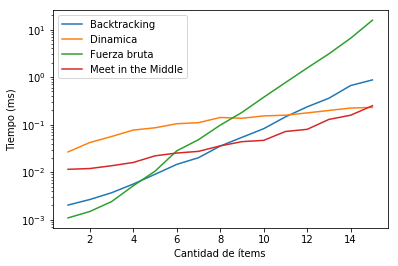
\includegraphics{capacidad100.png}

El gráfico muestra el tiempo tardado en milisegundos por cada algoritmo en una escala logarítmica. Se probó cada uno con 100 combinaciones de ítems para cada cantidad de 0 a 15, con una capacidad de la mochila de 100. Los tamaños y beneficios de los ítems se generaron con una variable aleatoria de distribución uniforme de 0 a 10 inclusive.\par
Como podemos ver, el algoritmo de Fuerza Bruta sigue bastante fielmente un crecimiento exponencial del tiempo tardado según crece la cantidad de ítems. El algoritmo de Meet in the Middle parece crecer más lentamente que los demás, hasta que se llega a los 15 ítems, en el que sobrepasa en tiempo al de dinámica, aunque este único gráfico no nos aporta suficiente información. El de Backtracking parece sostener un crecimiento exponencial constante, como el de Fuerza Bruta, y el de Dinámica se estanca en comparación a los otros después del primer salto entre 0 ítems y 1 ítem. Podemos suponer que esto se debe a que la complejidad no crece tanto con la cantidad de ítems como los otros, y que con 0 ítems la tabla que se crea es de tamaño 0, mientras que la tabla que se crea con 1 ítem es de tamaño igual a la capacidad.\par

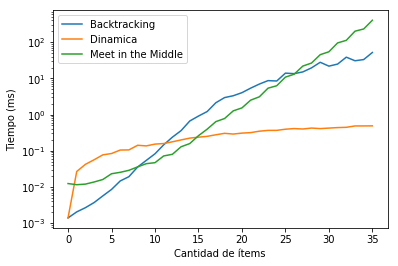
\includegraphics{capacidad100sinfuerza.png}

Este gráfico es una extensión del gráfico anterior, pero omitiendo los tiempos tardados por el algoritmo de Fuerza Bruta, por ser ya demasiado grandes. Además, el hecho de aumentar la cantidad de ítems también incrementa la varianza de los resultados, así que se hace un muestreo de 300 combinaciones en vez de 100. Podemos ver que el algoritmo de dinámica casi no crece en comparación a los otros dos, y, como dijimos antes, que el de Meet in the Middle pierde la ventaja que tenía al principio después de los 15 elementos, para perder incluso contra el de Backtracking. Parecería, según los datos, que las podas del algoritmo de backtracking ganan fuerza cuanto más elementos hay, porque se puede ver un crecimiento más lento de los tiempos luego de los 20 elementos. También podemos ver que sus valores varían más, como dijimos en nuestras hipótesis. En donde no se cumplen nuestras hipótesis es en la relación entre el Backtracking y el Meet in the Middle: aunque estuvieron medianamente empatados hasta los 25 elementos, cuando se agregan más el de Backtracking mejora bastante los tiempos, tomando en cuenta de que el gráfico está en una escala logarítmica.\par
Ahora analizaremos el incremento de tiempos para el algoritmo de Dinámica cuando crece la capacidad de la mochila.\par
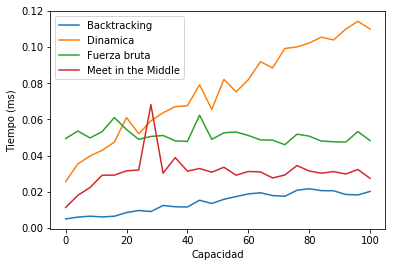
\includegraphics{aumentocapacidad.png}

Este gráfico se produjo tomando una granuralidad de 4 en la capacidad de la mochila, con 100 muestras de 7 ítems en cada paso. Como previmos, el tiempo que tarda el algoritmo de Dinámica crece con la capacidad de la mochila, mientras que los otros algoritmos mantienen su desempeño. Los que también crecen un poco son los de Meet in the Middle y de Backtracking, por el hecho de que los dos descartan combinaciones si es que el tamaño supera la capacidad. Al aumentar la capacidad, hay menos combinaciones que se pueden descartar rápidamente.\par
En conclusión, el algoritmo de Backtracking parece ser el mejor en promedio cuando se tiene poca cantidad de ítems y mucha capacidad, y el de dinámica parece ser el mejor cuando pasa lo contrario. Por lo visto en los gráficos, el algoritmo de dinámica crece mucho más lento con la capacidad que los demás con la cantidad de ítems, así que a lo que nos referimos con poca cantidad, por lo menos con una capacidad de 100, sería menos de 15.
\end{document}
